\section{问题一:关系模型的建立与求解}
为识别影响男胎 Y 染色体浓度的主要因素并量化其作用,我们先构建最终数据集,再通过探索性分析与迭代建模建立能反映数据结构的关系模型。流程见 \cref{fig:关系模型的建立与求解流程}。

\begin{figure}[h]
	\centering
	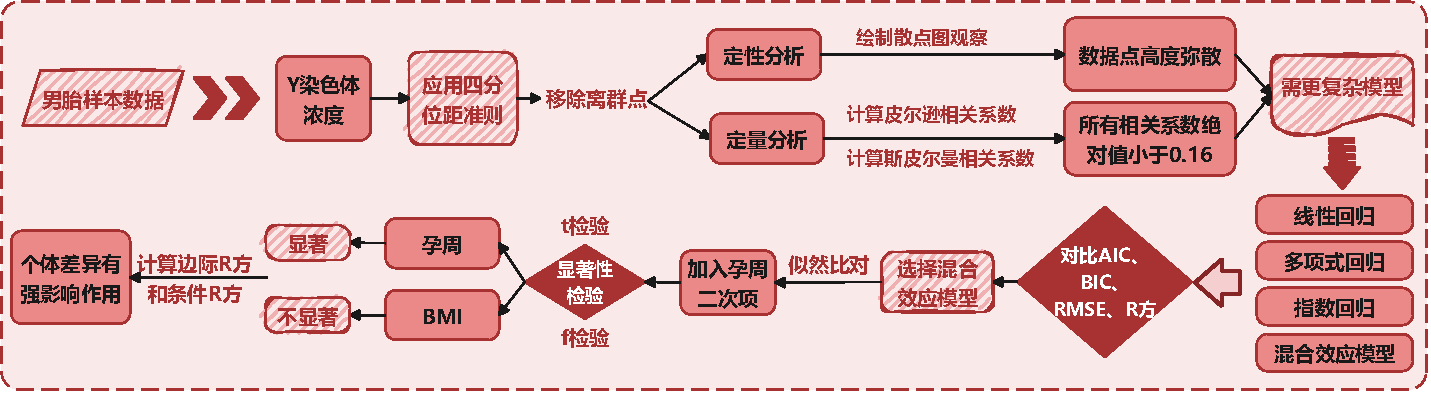
\includegraphics[width=\textwidth]{figs/3问题一/问题一.pdf}
	\caption{关系模型的建立与求解流程}
	\label{fig:关系模型的建立与求解流程}
\end{figure}

\subsection{分析数据集的构建}
本文的分析始于经过初步处理的男胎样本数据。为保证模型的稳健性,避免极端值对模型参数估计产生不当影响,我们对Y染色体浓度,孕妇BMI,年龄与孕周四个核心变量应用了1.5倍四分位距准则进行离群点检测。该准则将分布于数据主体之外的极端观测值识别为离群点。在联合筛选过程中,任何在上述四个变量中至少存在一个离群点的样本记录均被移除。经过筛选,共54条记录被剔除,最终形成了包含944条高质量观测记录的分析数据集。该数据清洗过程的效果如\cref{fig:Y浓度离群点剔除可视化}所示,图中展示了Y染色体浓度变量在离群点剔除前后的分布变化,处理后的数据分布更为集中,减少了极端值可能带来的干扰。

\begin{figure}[h!]
	\centering
	\begin{minipage}[b]{0.48\textwidth}
		\centering
		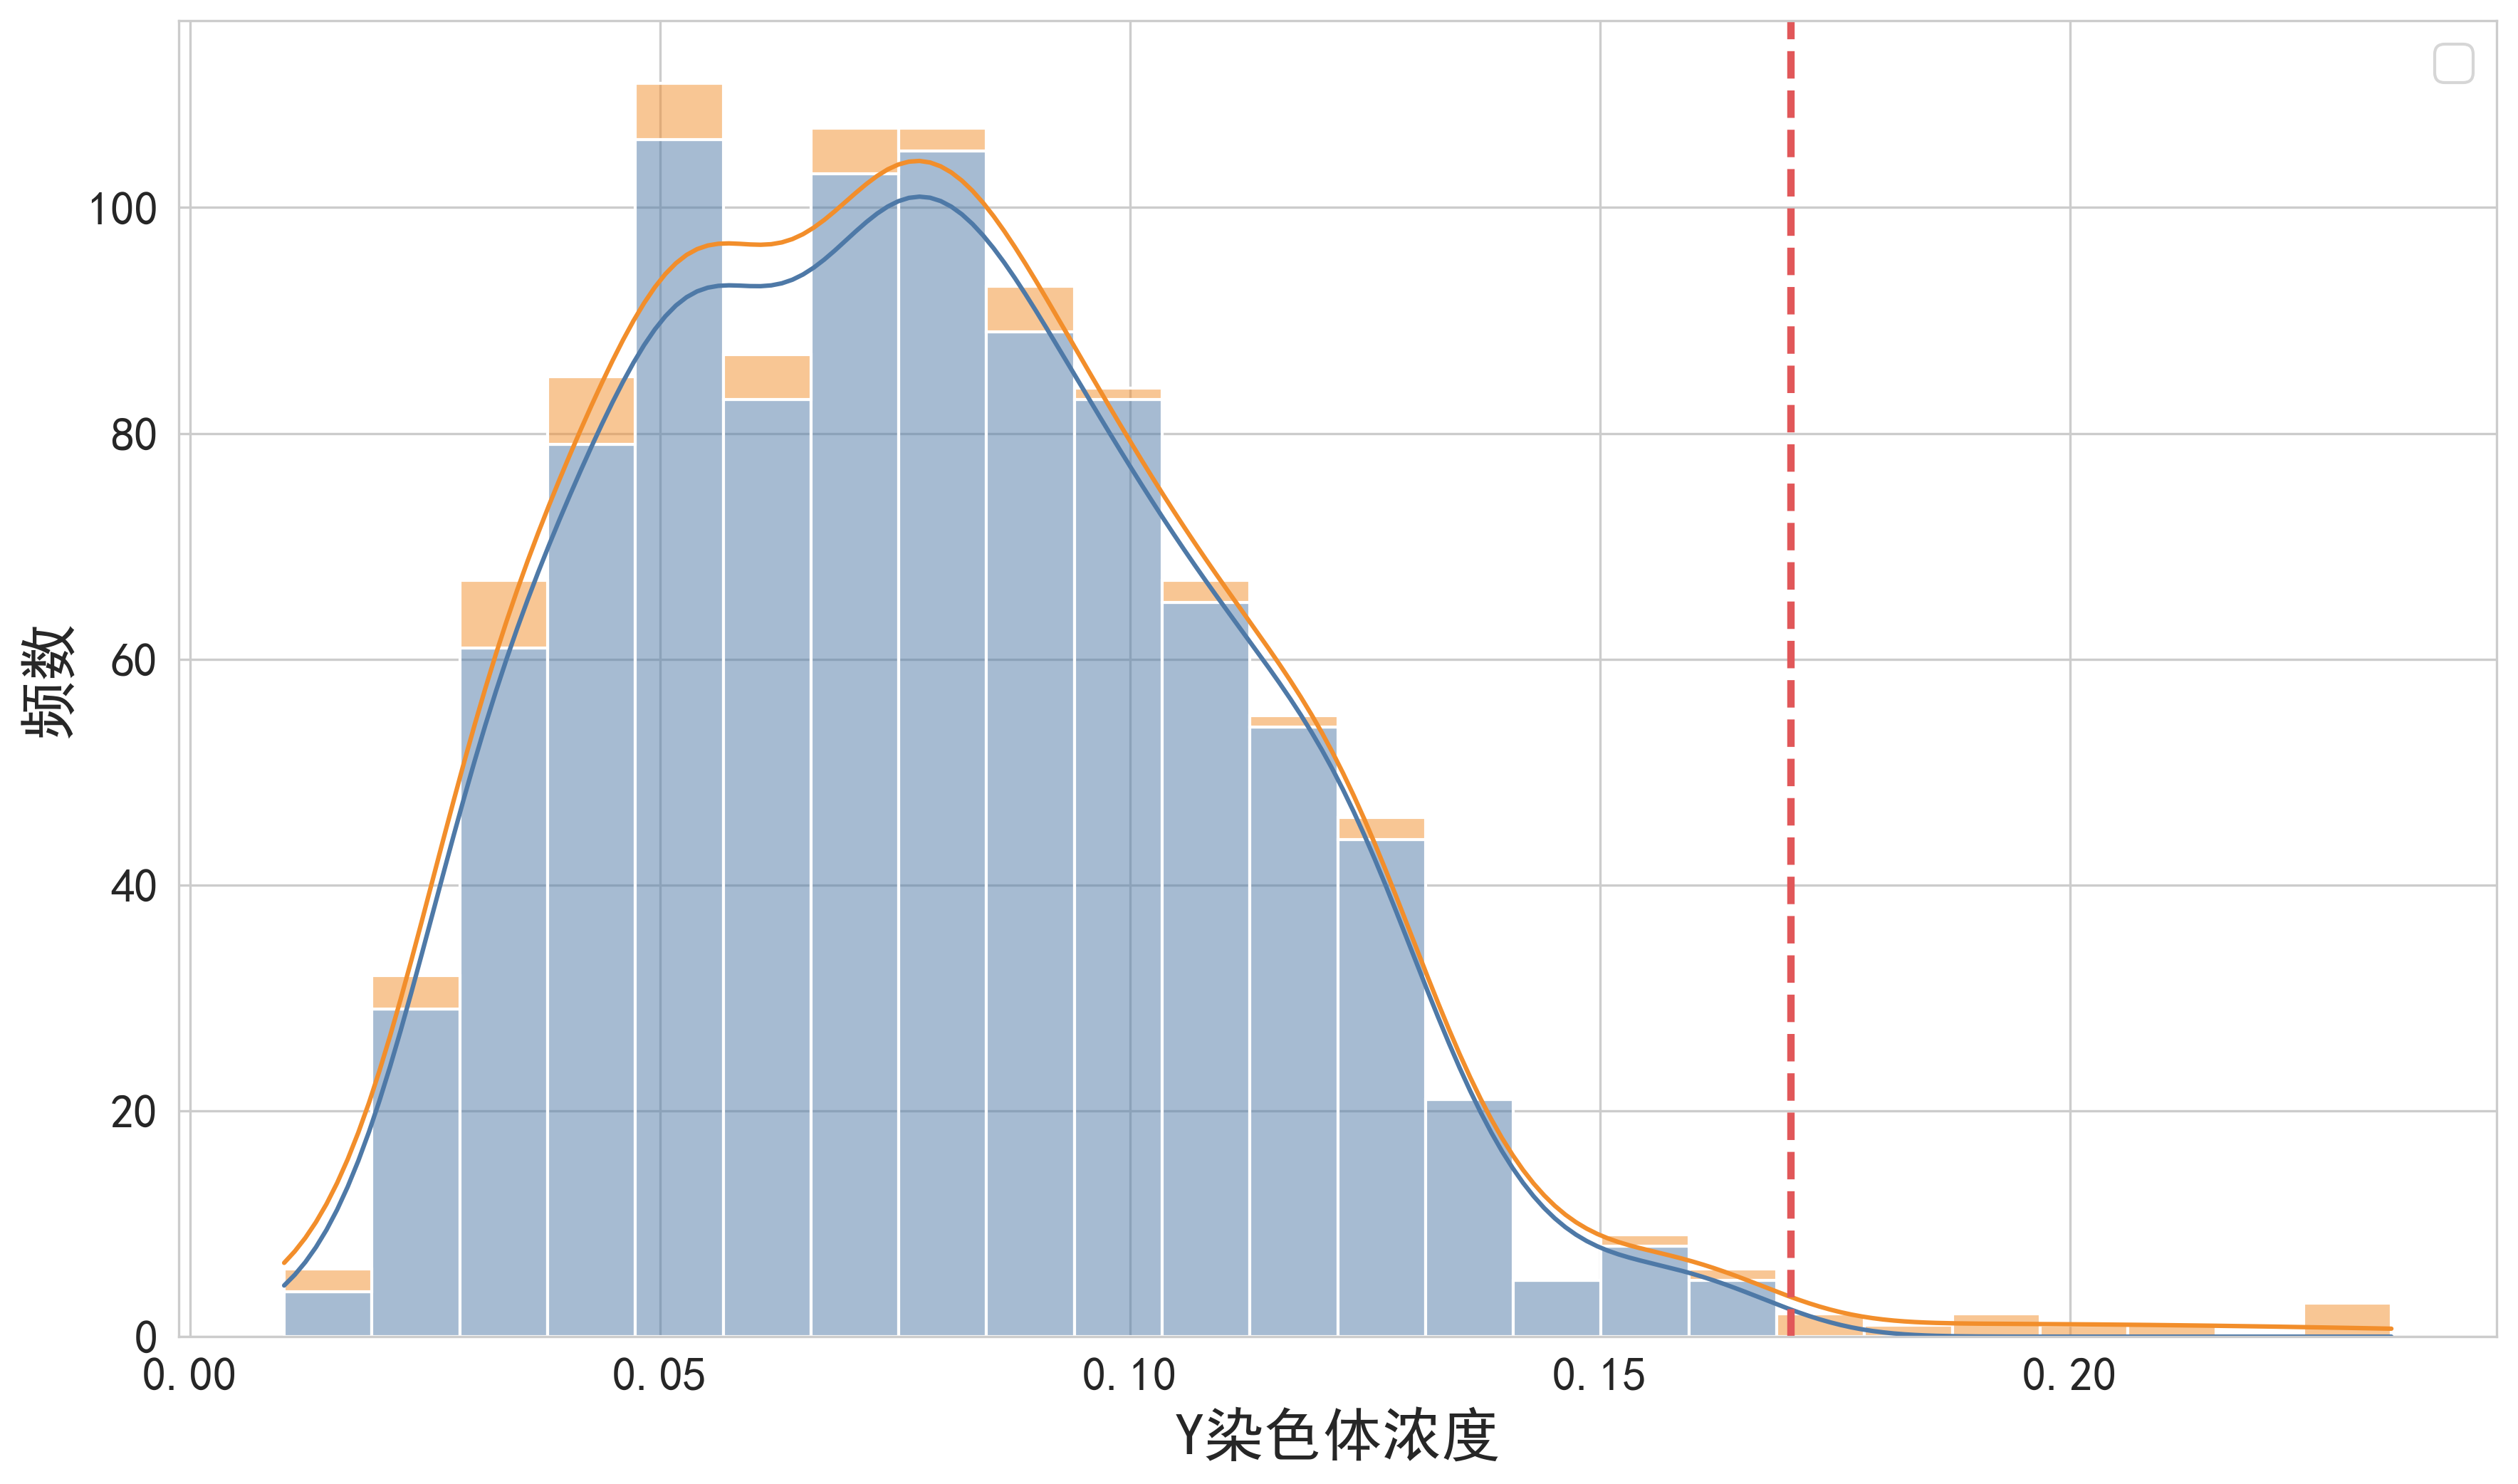
\includegraphics[width=1\textwidth]{figs/3问题一/图1_Y浓度离群点剔除可视化.png}
		\caption{Y染色体浓度离群点剔除前后对比}
		\label{fig:Y浓度离群点剔除可视化}
	\end{minipage}
	\hfill
	\begin{minipage}[b]{0.48\textwidth}
		\centering
		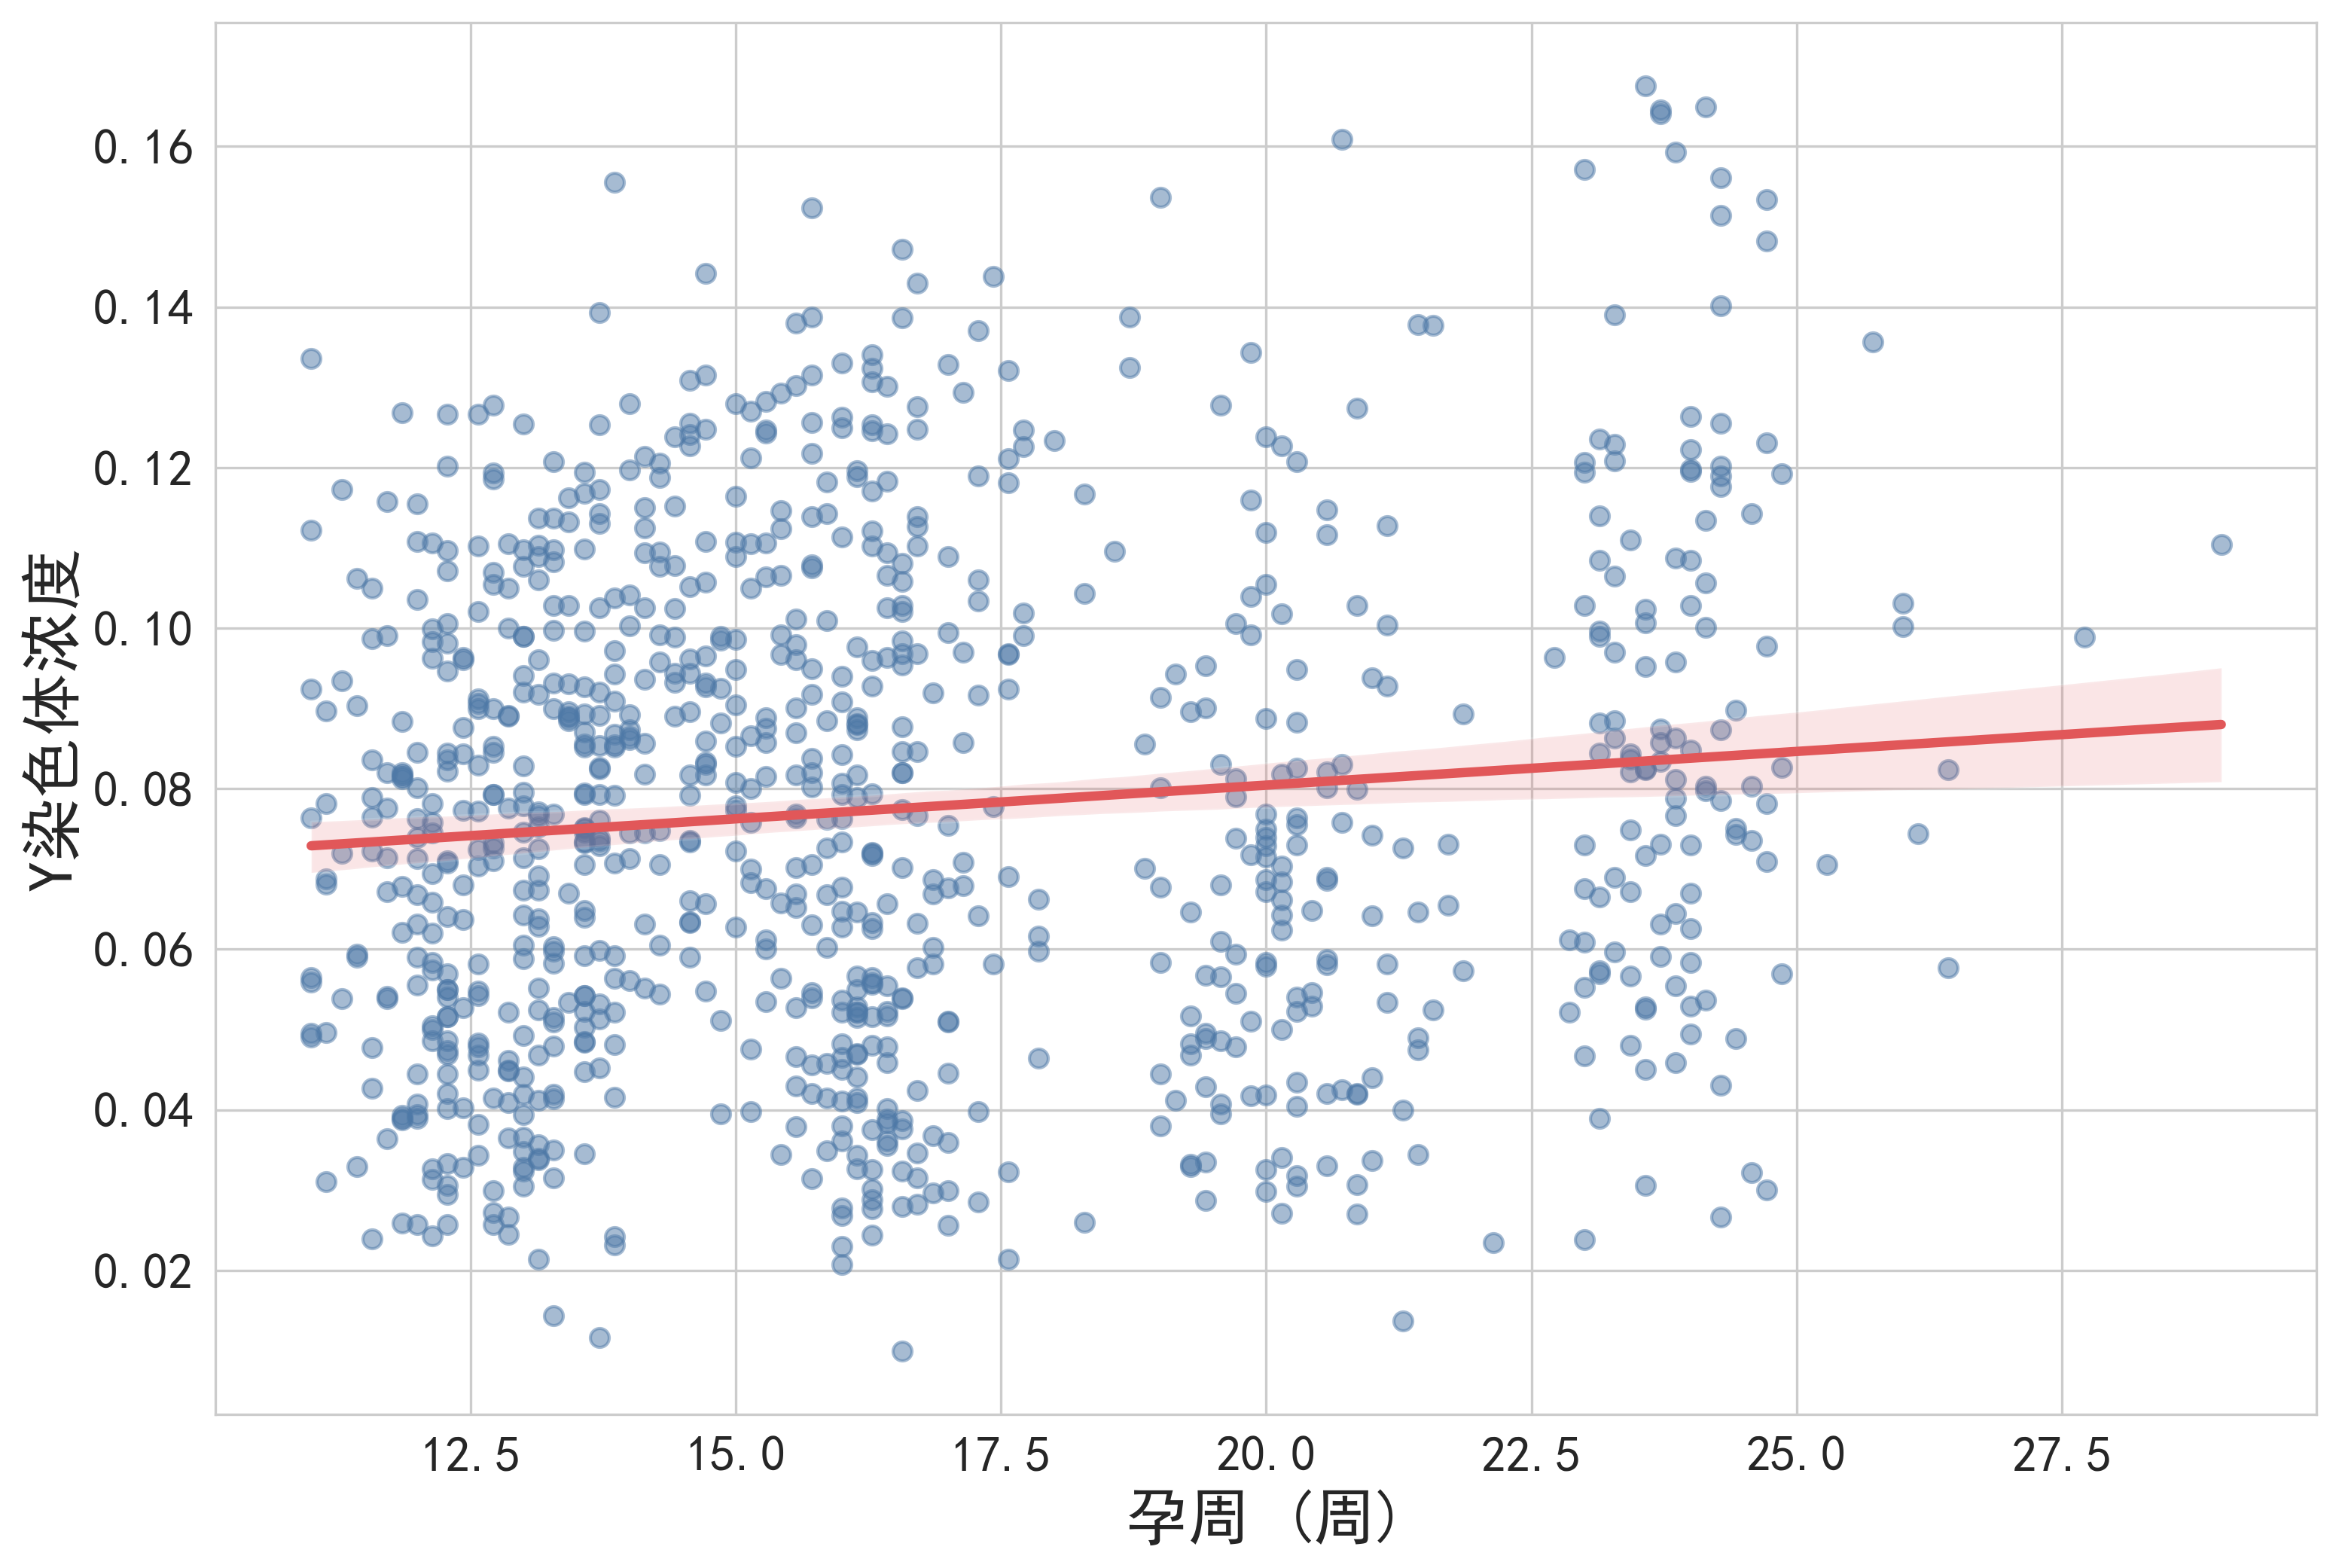
\includegraphics[width=\textwidth]{figs/3问题一/图3_Y浓度_vs_孕周_散点图.png}
		\caption{Y染色体浓度与孕周}
		\label{fig:Y浓度_vs_孕周_散点图}
	\end{minipage}
	\hfill
	\begin{minipage}[b]{0.48\textwidth}
		\centering
		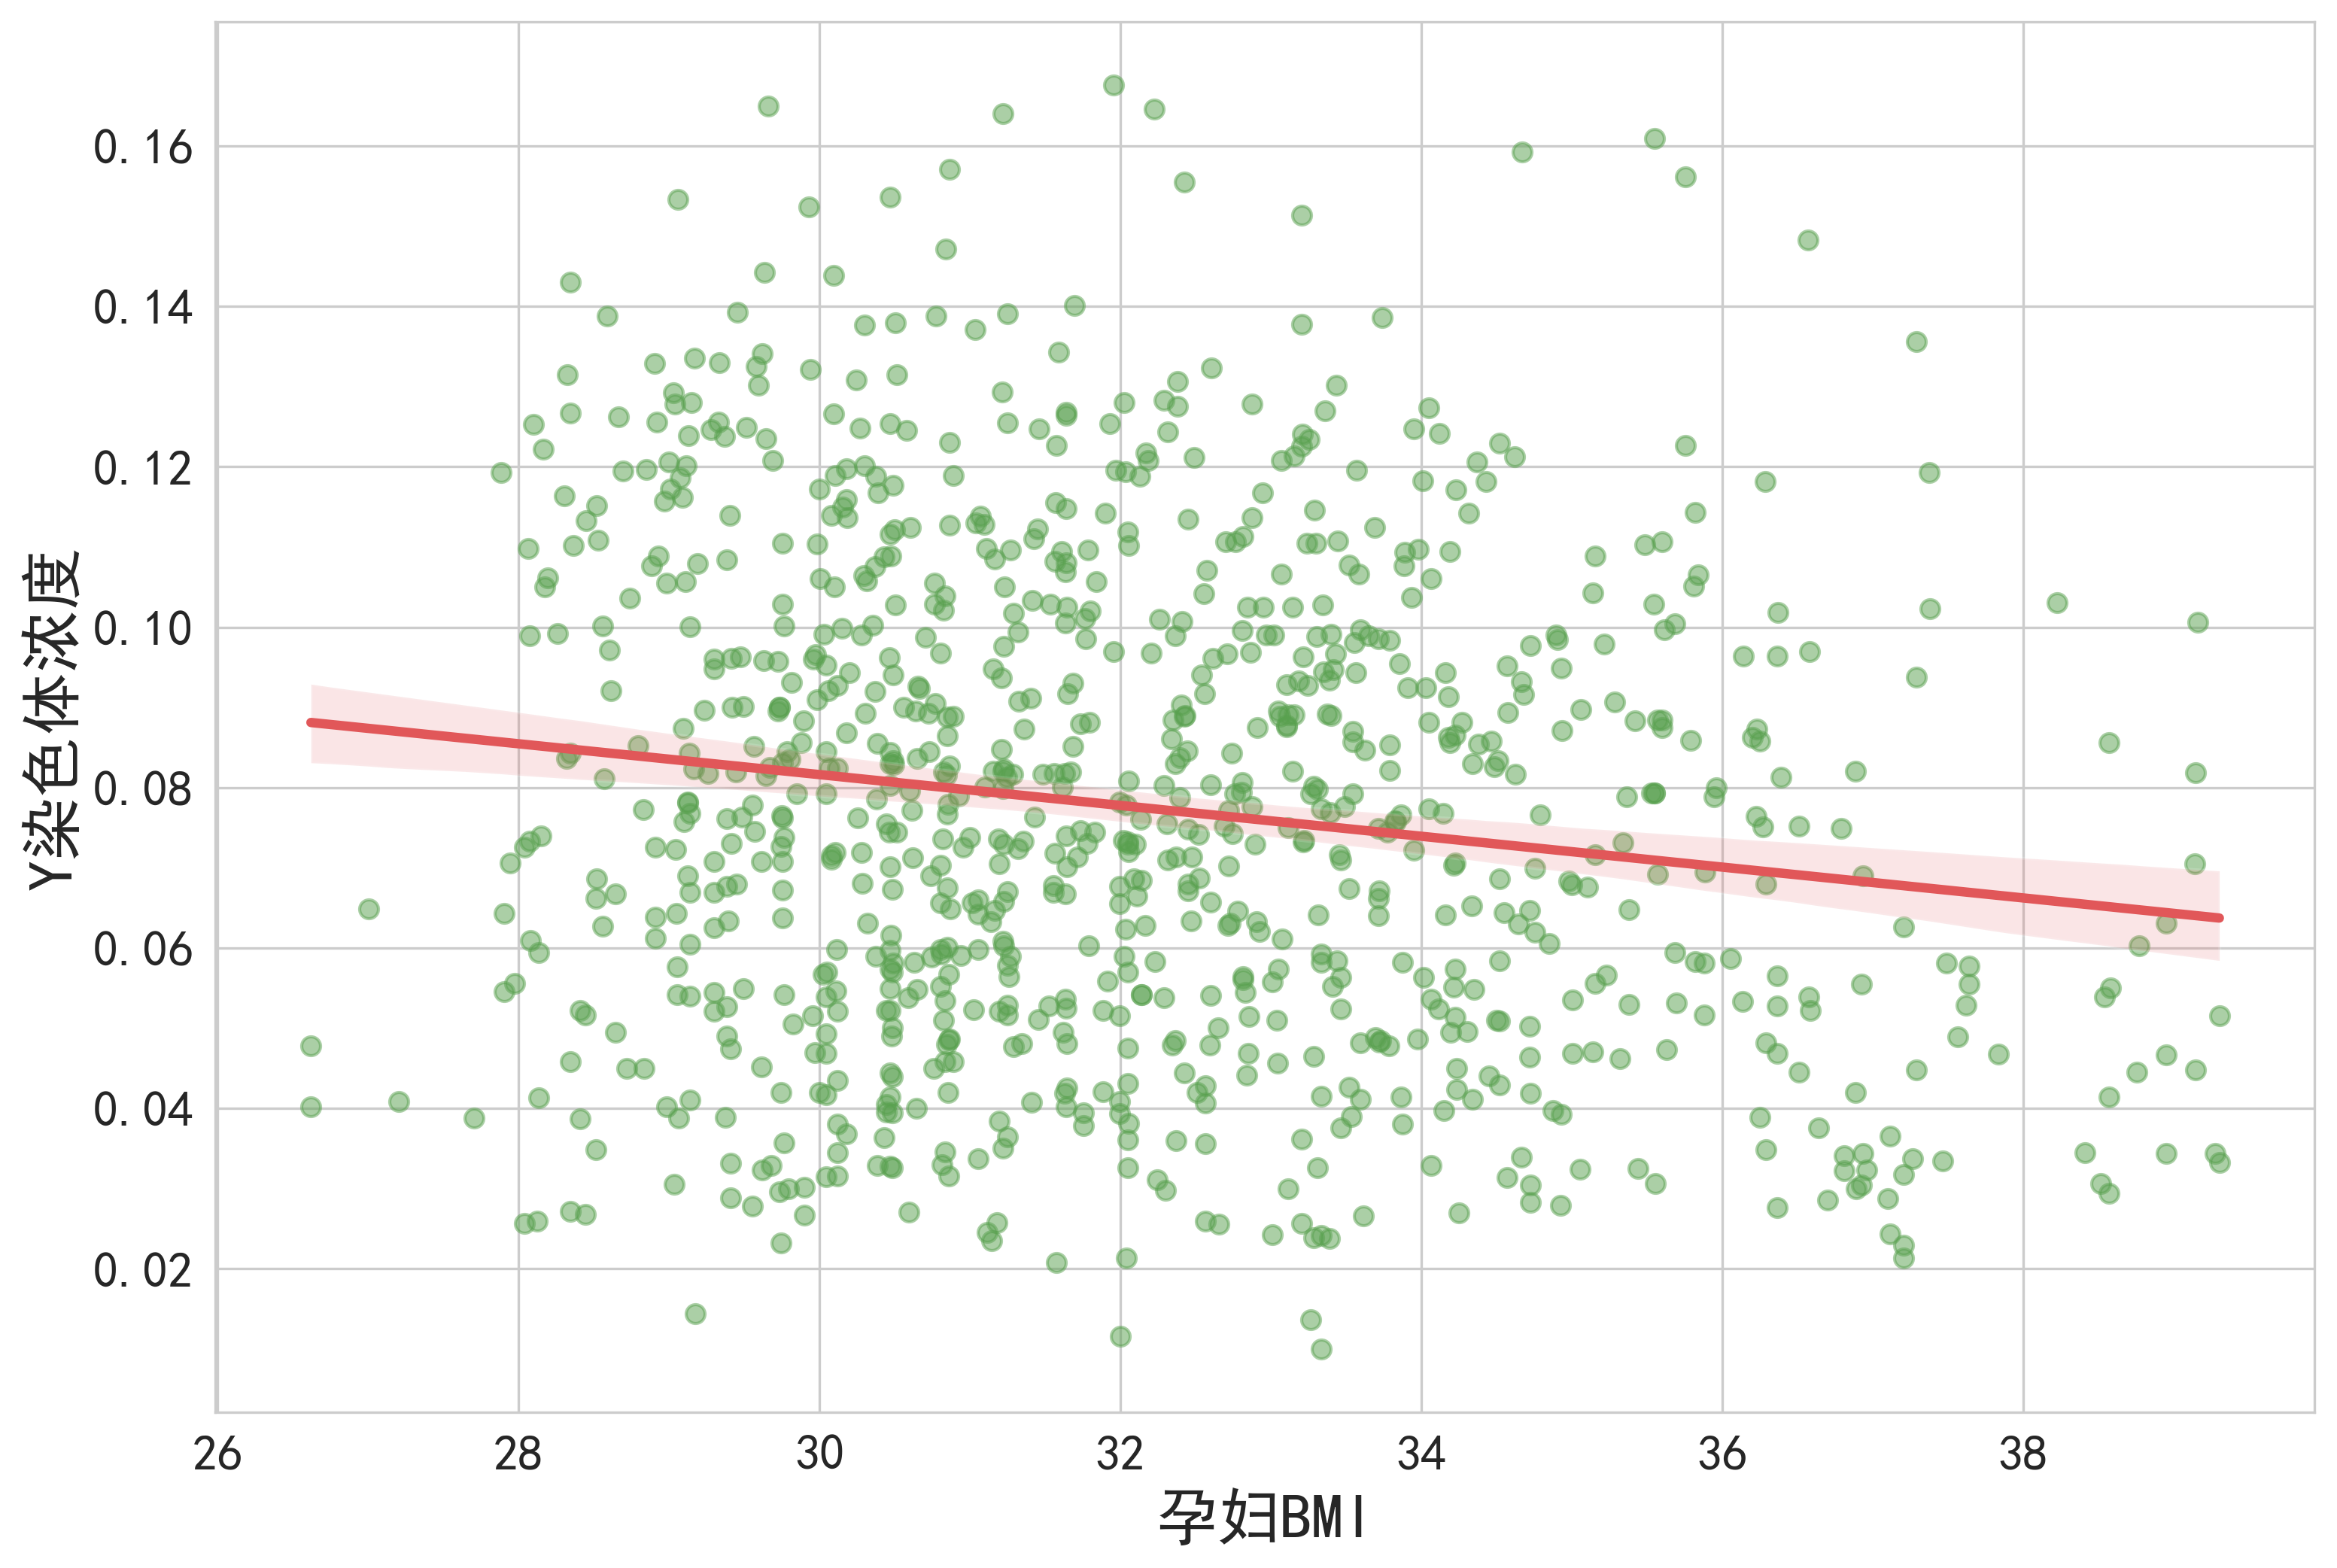
\includegraphics[width=\textwidth]{figs/3问题一/图4_Y浓度_vs_孕妇BMI_散点图.png}
		\caption{Y染色体浓度与孕妇BMI}
		\label{fig:Y浓度_vs_孕妇BMI_散点图}
	\end{minipage}
	\hfill
	\begin{minipage}[b]{0.48\textwidth}
		\centering
		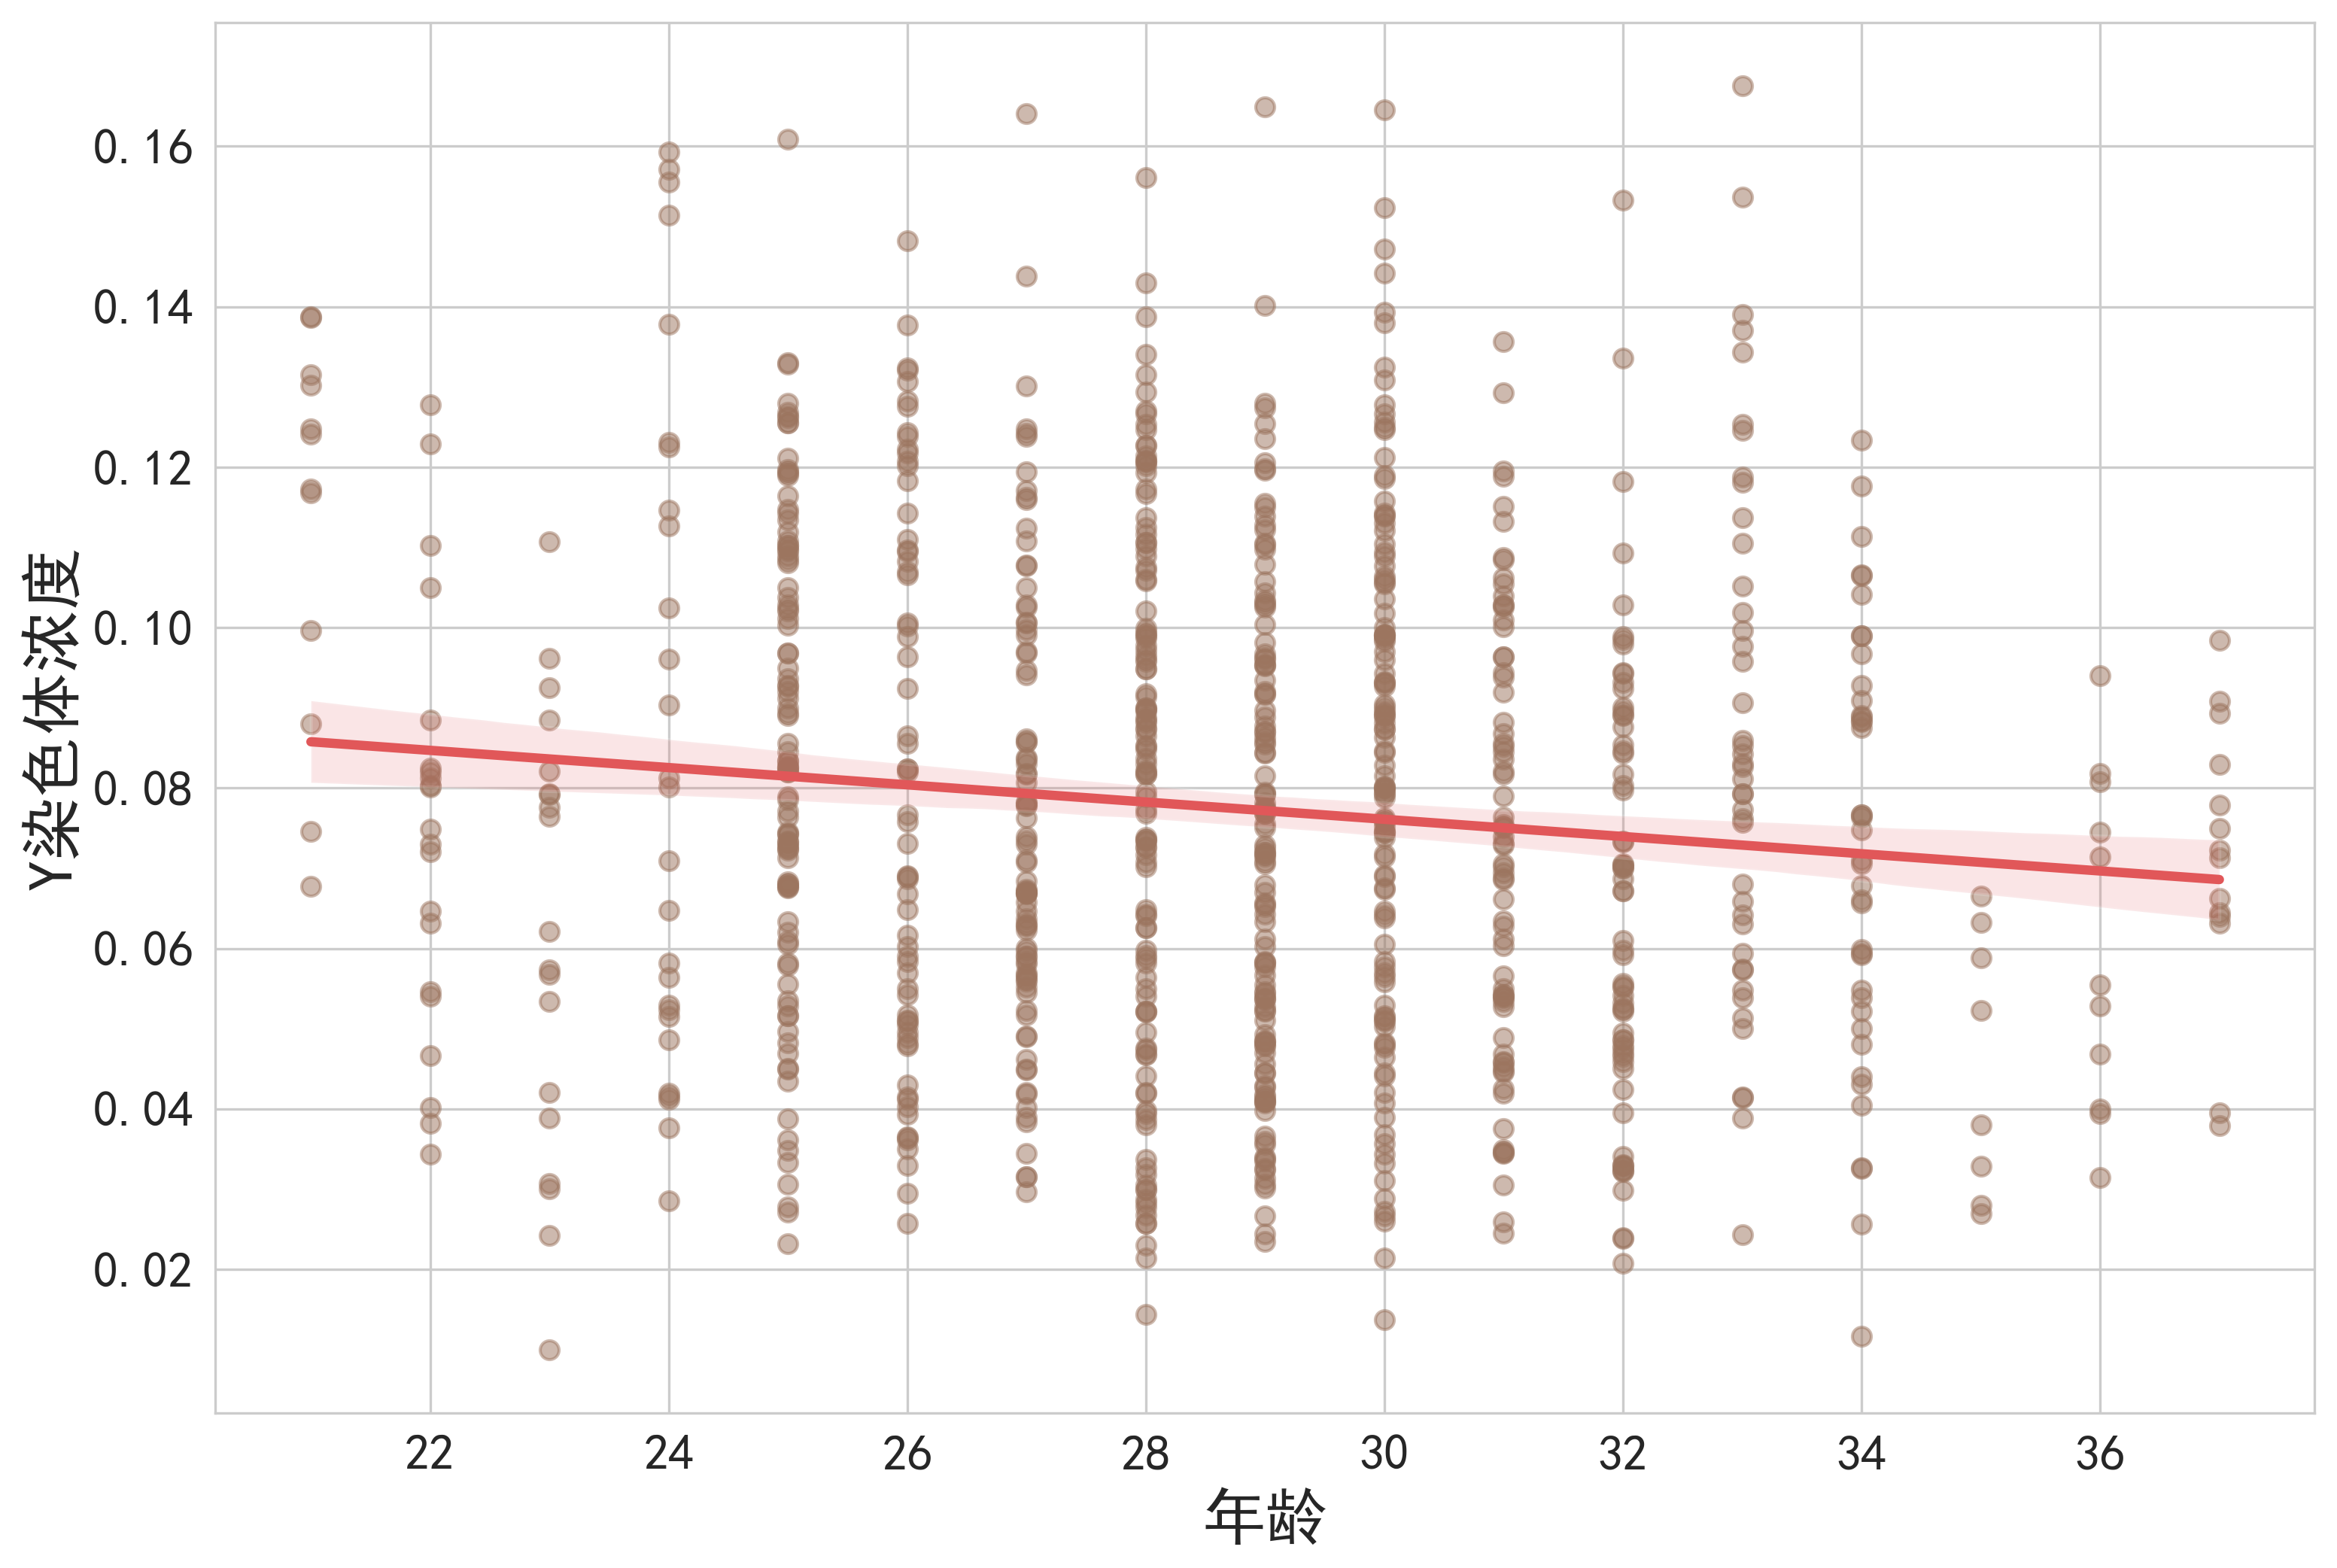
\includegraphics[width=\textwidth]{figs/3问题一/图5_Y浓度_vs_年龄_散点图.png}
		\caption{Y染色体浓度与年龄}
		\label{fig:Y浓度_vs_年龄_散点图}
	\end{minipage}
\end{figure}


\subsection{变量间关系的初步探索}
在进行正式的定量建模之前,有必要对变量间的关系形态进行初步的定性判断。我们绘制了Y染色体浓度分别与孕周,孕妇BMI及年龄的散点图。如\cref{fig:Y浓度_vs_孕周_散点图},\cref{fig:Y浓度_vs_孕妇BMI_散点图}与\cref{fig:Y浓度_vs_年龄_散点图}所示,在所有散点图中,数据点均呈现高度弥散的分布状态,并未形成任何可被简单函数描述的清晰模式。


为对上述视觉观察进行量化确认,我们计算了核心变量间的相关性。本文采用皮尔逊相关系数与斯皮尔曼相关系数两种方法评估变量间的关联程度。皮尔逊相关系数用以衡量变量间的线性关系,其计算方法如下
\begin{equation}
	r = \frac{\sum_{i=1}^{n}(x_i - \bar{x})(y_i - \bar{y})}{\sqrt{\sum_{i=1}^{n}(x_i - \bar{x})^2} \sqrt{\sum_{i=1}^{n}(y_i - \bar{y})^2}}
\end{equation}
其中$x_i$与$y_i$为样本观测值,$\bar{x}$与$\bar{y}$为样本均值。斯皮尔曼相关系数则用于衡量变量间的单调关系,对变量的分布不作要求,其计算方法为
\begin{equation}
	\rho = 1 - \frac{6 \sum_{i=1}^{n} d_i^2}{n(n^2 - 1)}
\end{equation}
此处$d_i$为第$i$个样本在两个变量中的等级差值,$n$为样本量。如\cref{tab:相关性分析汇总表}的数值所示,Y染色体浓度与孕周呈微弱正相关,与孕妇BMI和年龄则呈微弱负相关。所有相关系数的绝对值均未超过0.16,这表明变量间的线性关系强度非常有限。初步探索的结论是,任何试图用单一自变量解释Y染色体浓度的简单模型都难以获得满意的结果,数据内部可能存在更为复杂的结构。

\begin{table}[h!]
	\centering
	\caption{相关性分析汇总表}
	\label{tab:相关性分析汇总表}
	\begin{tabular}{ccc}
		\hline
		变量对       & 皮尔逊相关系数 (r) & 斯皮尔曼相关系数 (ρ) \\
		\hline
		浓度 vs 孕周  & 0.1069      & 0.0837       \\
		浓度 vs BMI & -0.1558     & -0.1339      \\
		浓度 vs 年龄  & -0.1141     & -0.1008      \\
		\hline
	\end{tabular}
\end{table}

\subsection{关系模型的选择与确立}
考虑到变量间简单的线性关系较弱,本文通过建立与比较一系列数学模型,以期找到最能反映数据规律的模型。我们考察了四种候选模型,包括标准线性回归模型M1,多项式回归模型M2,指数回归模型M3,以及混合效应模型M4。其数学形式如下。

模型M1为标准多元线性回归模型
\begin{equation}
	Y_{ij} = \beta_0 + \beta_1 \text{GW}_{ij} + \beta_2 \text{BMI}_{ij} + e_{ij}
\end{equation}

模型M2为多元多项式回归模型
\begin{equation}
	Y_{ij} = \beta_0 + \sum_{k=1}^p \beta_k \text{GW}_{ij}^k + \sum_{l=1}^q \gamma_l \text{BMI}_{ij}^l + e_{ij}
\end{equation}

模型M3为多元指数回归模型
\begin{equation}
	\ln(Y_{ij}) = \beta_0 + \beta_1 \text{GW}_{ij} + \beta_2 \text{BMI}_{ij} + e_{ij}
\end{equation}

模型M4为混合效应模型
\begin{equation}
	Y_{ij} = (\beta_0 + u_{0i}) + \sum_{k=1}^p \beta_k \text{GW}_{ij}^k + \sum_{l=1}^q \gamma_l \text{BMI}_{ij}^l + e_{ij}
\end{equation}
其中$Y_{ij}$为因变量,GW与BMI为自变量,$e_{ij}$为误差项。$u_{0i}$项为第$i$个体的随机截距,服从均值为0,方差为$\sigma_u^2$的正态分布。

为对上述模型进行评估,我们采用了系数显著性检验与联合显著性检验。系数显著性检验用于判断模型中单个自变量的有效性,其t统计量的计算方式为
\begin{equation}
	t = \frac{\hat{\beta}_k}{SE(\hat{\beta}_k)}
\end{equation}
其中$\hat{\beta}_k$为系数估计值,$SE(\hat{\beta}_k)$为其标准误。联合显著性检验则用于判断模型所有自变量在整体上是否有效,其F统计量的计算方式为
\begin{equation}
	F = \frac{SSR/k}{SSE/(n-k-1)}
\end{equation}
其中SSR为回归平方和,SSE为残差平方和,$n$为样本量,$k$为自变量个数。

\begin{table}[h!]
	\centering
	\caption{候选模型评估对比表}
	\label{tab:模型评估对比表}
	\begin{tabular}{ccccc}
		\hline
		模型         & 对数似然值   & AIC      & BIC      & RMSE \\
		\hline
		M1: 线性回归   & 1971.6  & -3935.2  & -3915.8  & 0.03 \\
		M2: 多项式回归  & 1971.84 & -3933.68 & -3909.43 & 0.03 \\
		M3: 指数回归   & -558.4  & 1124.8   & 1144.2   & 0.03 \\
		M4: 混合效应模型 & 2235.53 &     -     &     -     & 0.03 \\
		\hline
	\end{tabular}
\end{table}

模型的选择依据对数似然值,赤池信息准则AIC与贝叶斯信息准则BIC等指标进行,如\cref{tab:模型评估对比表}所示。在模型筛选过程中,M3因拟合效果最差被首先排除。M2模型中孕周的二次项系数在统计上不显著,且其AIC值劣于更为简洁的M1模型,故也被排除。在M1与M4的比较中,M4的对数似然值2235.53远高于M1的1971.6,说明M4模型能够更好地解释数据的变异性。标准线性回归模型M1的调整后决定系数仅为0.049,无法充分解释数据变异。混合效应模型通过引入随机效应来解释由个体差异引起的变异,在拟合优度上取得了大幅提升。综合考量,混合效应模型M4被确立为最终的关系模型。

\subsection{模型结果与显著性检验}
最终确立的混合效应模型能够将Y染色体浓度的变化分解为所有样本共有的固定效应部分和每个孕妇独有的随机效应部分。基于显著性检验结果,最终模型采用线性形式,其数学表达式如下
\begin{equation}
	\hat{Y}_{ij} = (\beta_0 + u_{0,i}) + \beta_1 \cdot \text{孕周}_{ij} + \beta_2 \cdot \text{BMI}_{ij} + \beta_3 \cdot \text{年龄}_{ij}
	\label{eq:mixed_model}
\end{equation}
其中$\hat{Y}_{ij}$代表第$i$位孕妇在第$j$次检测时的Y染色体浓度预测值。$\beta_0, \beta_1, \beta_2, \beta_3$是固定效应系数,代表了群体的平均趋势。$u_{0,i}$是随机效应部分,代表第$i$位孕妇的基础浓度与群体平均水平的偏离量。

为评估模型的解释能力,我们计算了模型的边际R方与条件R方。边际R方表示仅由固定效应即孕周,BMI与年龄解释的方差比例,而条件R方表示由固定效应和随机效应即个体差异共同解释的方差比例。
\begin{table}[h!]
	\centering
	\caption{混合效应模型R方统计量}
	\label{tab:R方统计量}
	\begin{tabular}{cc}
		\hline
		指标                     & 值     \\
		\hline
		边际 R² & 0.1352 \\
		条件 R² & 0.7727 \\
		\hline
	\end{tabular}
\end{table}

\begin{table}[h!]
	\centering
	\caption{混合效应模型固定效应参数估计与显著性检验}
	\label{tab:M4固定效应参数表}
	\begin{tabular}{ccccc}
		\hline
		参数        & 系数估计值  & 标准误   & z值     & p值    \\
		\hline
		Intercept & 0.102  & 0.024 & 4.207  & 0.000 \\
		孕周        & 0.003  & 0.000 & 17.672 & 0.000 \\
		孕妇BMI     & -0.001 & 0.001 & -2.309 & 0.021 \\
		年龄        & -0.001 & 0.001 & -1.870 & 0.062 \\
		\hline
	\end{tabular}
\end{table}

\cref{tab:R方统计量}的R方值表明,模型的固定效应部分可解释约13.5\%的Y染色体浓度变异,而在计入个体差异的随机效应后,模型总共可以解释约77.3\%的变异。\cref{tab:M4固定效应参数表}展示了模型固定效应的参数估计及其显著性检验结果。对于每个参数,我们检验其系数是否为零的原假设。在0.05的显著性水平下,孕周的p值为0.000,远小于0.05,故拒绝原假设,认为孕周对Y染色体浓度存在统计上显著的正向影响。孕妇BMI的p值为0.021,小于0.05,同样拒绝原假设,认为孕妇BMI存在统计上显著的负向影响。年龄的p值为0.062,大于0.05,因此不能拒绝原假设,认为在当前模型中未发现年龄有统计上显著的影响。

\begin{figure}[h!]
	\centering
	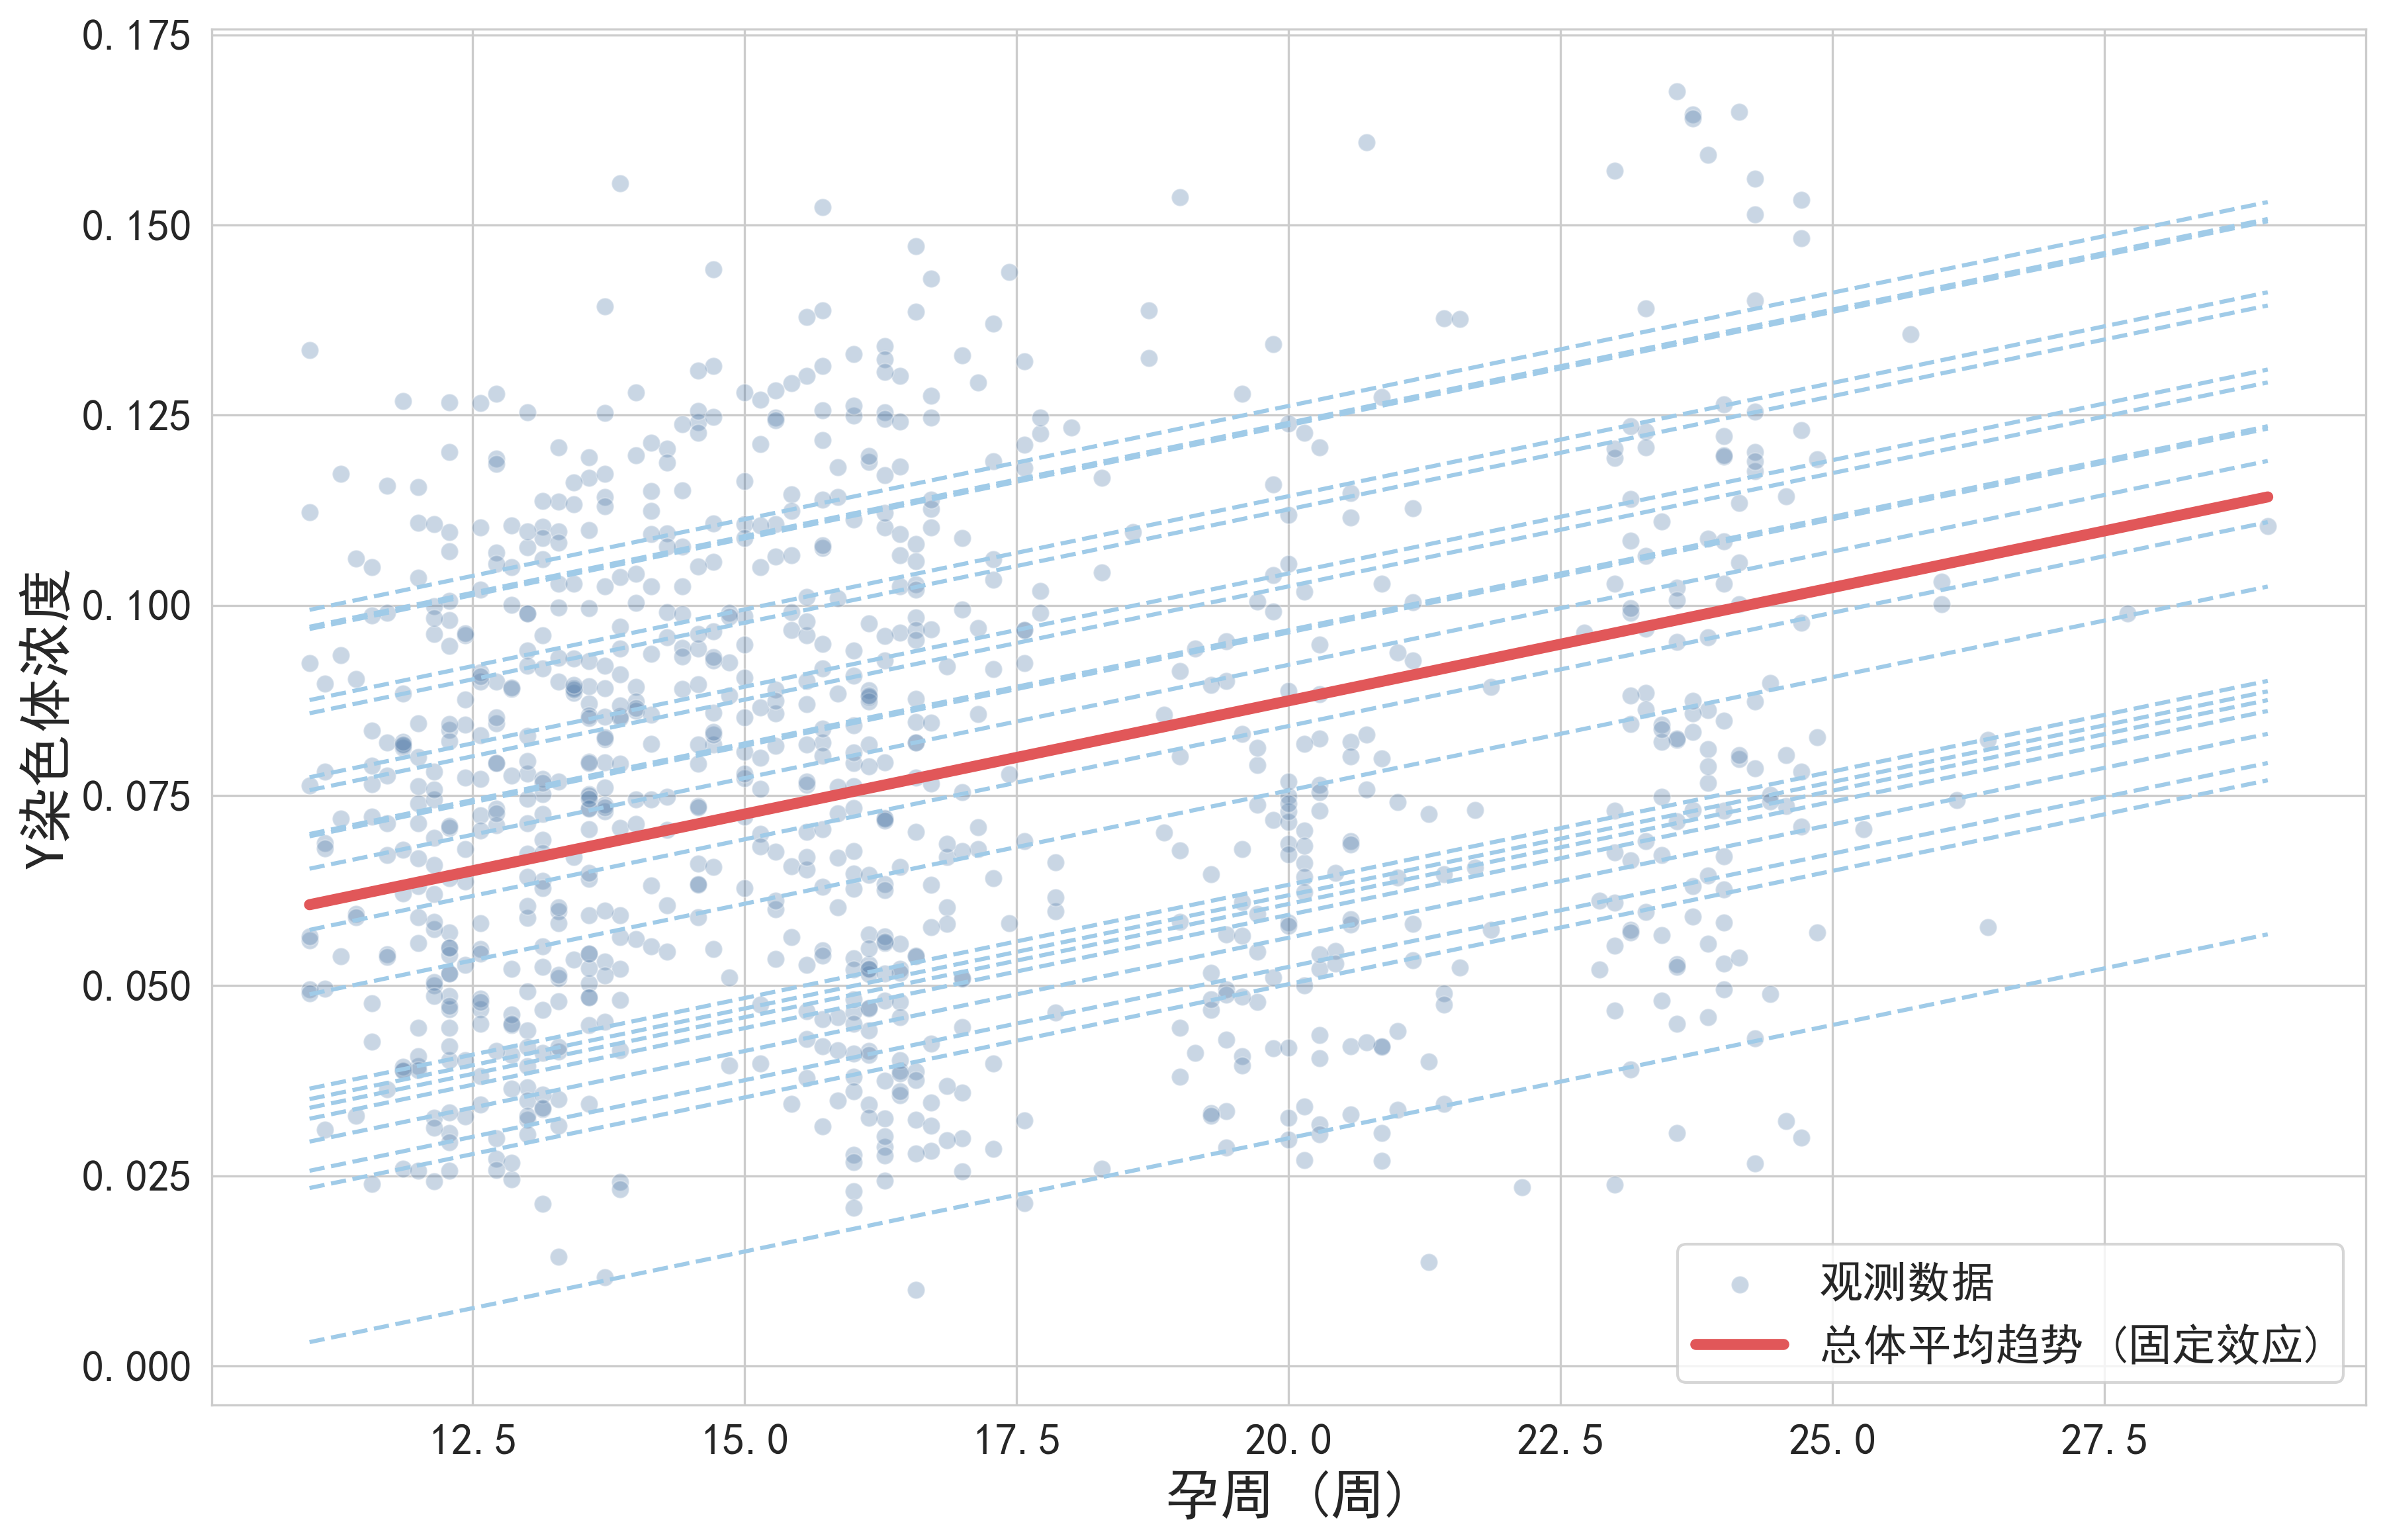
\includegraphics[width=1\textwidth]{figs/3问题一/图6_最终模型M4_可视化.png}
	\caption{混合效应模型可视化}
	\label{fig:最终模型M4_可视化}
\end{figure}

\cref{fig:最终模型M4_可视化}展示了模型结果。图中的红色实线代表了由固定效应决定的群体平均增长趋势,而大量的蓝色虚线则描绘了不同孕妇个体的实际浓度变化轨迹。这直观地体现了固定效应所代表的普遍规律与随机效应所代表的个体差异。

综上所述,通过显著性检验,我们确立了Y染色体浓度与孕妇部分指标的关系。Y染色体浓度随孕周增长而显著上升,随孕妇BMI的增加而显著下降。此外,不同孕妇之间的个体差异是影响浓度的重要因素,但未发现年龄有统计上显著的影响。